\section{Contraste con las cifras oficiales}\label{sec:siap}

Si la brecha fuera una característica de la zona, aparecería también en la estadística oficial de esos municipios.
Para comprobarlo comparamos la media del reto de cada municipio con el rendimiento del cierre agrícola del SIAP de
2023, 2024 y 2025 (Fig.~\ref{fig:siap}).

\begin{figure}[t]
\centering
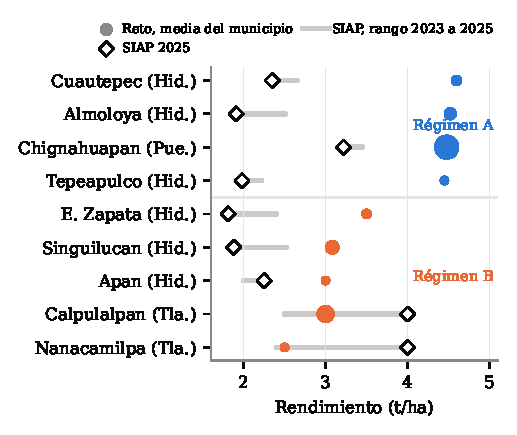
\includegraphics[width=\columnwidth]{r6_siap}
\caption{Rendimiento medio del reto por municipio (círculos, tamaño según el número de parcelas) contra el
rendimiento oficial del SIAP para cebada grano de temporal, primavera-verano.}
\label{fig:siap}
\end{figure}

\begin{itemize}
\item \textbf{En el SIAP no hay brecha entre regímenes.} El promedio de 2023 a 2025 es 2.51\,t/ha en los municipios A
y 2.48 en los B. En el reto es 4.51 contra 3.02.
\item \textbf{En Hidalgo, dentro de la misma zona, los dos regímenes rinden igual.} En 2025, Almoloya, Cuautepec y
Tepeapulco (A) tuvieron 1.91, 2.35 y 1.98\,t/ha, y Singuilucan, Apan y Emiliano Zapata (B) tuvieron 1.88, 2.25 y
1.81.
\item \textbf{En 2025, el SIAP muestra lo contrario del reto.} Calpulalpan y Nanacamilpa (B) tuvieron 4.00\,t/ha,
más que Chignahuapan (3.22). El reto les da 3.00 y 2.50 contra 4.48.
\item \textbf{Todo el régimen A queda muy por arriba de lo oficial.} Su media supera a la del SIAP 2025 de su
municipio entre 1.26 y 2.61\,t/ha. En el régimen B, la diferencia va de $-1.50$ a $+1.69$.
\item \textbf{El nivel oficial no predice las etiquetas.} La correlación entre la media del reto y la del SIAP por
municipio es $-0.43$ en 2025 y $-0.13$ en el promedio de los tres años. Usar el SIAP 2025 para predecir las parcelas
de un municipio nuevo da un RMSE de 1.47\,t/ha, peor que la media global (1.15).
\end{itemize}

El SIAP también tiene limitaciones. Es una estimación agregada de todos los productores del municipio, y en Tlaxcala
2025 trae valores redondos (4.00 y 5.00), señal de estimaciones. Aun así, es una fuente independiente que aplica el
mismo criterio a todos los municipios, y no reproduce la brecha.
